\documentclass[journal]{IEEEtran}
\usepackage[a5paper, margin=10mm, onecolumn]{geometry}
\usepackage{tfrupee} % Include tfrupee package
\usepackage{gvv-book}
\usepackage{gvv}
\usepackage{cite}
\usepackage{amsmath,amssymb,amsfonts,amsthm}
\usepackage{algorithmic}
\usepackage{graphicx}
\usepackage{textcomp}
\usepackage{xcolor}
\usepackage{txfonts}
\usepackage{booktabs}  % For professional-looking tables
\usepackage{array}
\usepackage{listings}
\usepackage{enumitem}
\usepackage{mathtools}
\usepackage{gensymb}
\usepackage{comment}
\usepackage{tkz-euclide}
\usepackage{circuitikz}
\usepackage{array}
\usepackage{longtable}
\usepackage{multirow}
\usepackage{hhline}
\usepackage{ifthen}
\usepackage{lscape}
\usepackage{hyperref}

\hypersetup{breaklinks=true}

% Arduino code styling
\lstset{
    language=C++,
    basicstyle=\ttfamily\small,
    keywordstyle=\color{blue},
    commentstyle=\color{green},
    stringstyle=\color{red},
    numbers=left,
    numberstyle=\tiny\color{gray},
    stepnumber=1,
    numbersep=5pt,
    backgroundcolor=\color{white},
    showspaces=false,
    showstringspaces=false,
    showtabs=false,
    tabsize=2,
    captionpos=b,
    breaklines=true,
    breakatwhitespace=true,
    frame=single
}

\title{digital clock}
\author{Jadhav Rajesh-EE24BTECH11028}
\date{\today}

\begin{document}

\maketitle

\section{Objective}
The objective of this experiment is to design and implement a digital clock using an \textbf{Arduino} and the \textbf{7447 BCD to 7-segment decoder/driver IC}. The clock displays time in the \textbf{HH:MM:SS} format on six 7-segment displays. The Arduino generates the BCD (Binary-Coded Decimal) output, which is decoded by the 7447 IC to drive the 7-segment displays.

\section{Components Required}
\begin{itemize}
    \item Arduino Uno (or compatible board).
    \item Six 7-segment displays (common cathode or common anode).
    \item Six 7447 BCD to 7-segment decoder/driver ICs.
    \item Resistors $(220\Omega$ for current limiting in 7-segment displays).
    \item Breadboard and connecting wires.
    \item Power supply (5V DC from Arduino or external source).
    \item Push buttons (optional, for manual time setting).
\end{itemize}

\section{Circuit Design}
The digital clock is designed using the following components and connections:

\subsection{Arduino to 7447 IC}
\begin{itemize}
    \item Connect the 4 BCD output pins of the Arduino (e.g., D2, D3, D4, D5) to the BCD input pins (A, B, C, D) of the 7447 IC.
    \item Connect the GND pin of the Arduino to the GND pin of the 7447 IC.
\end{itemize}
\begin{figure}[H]
    \centering
    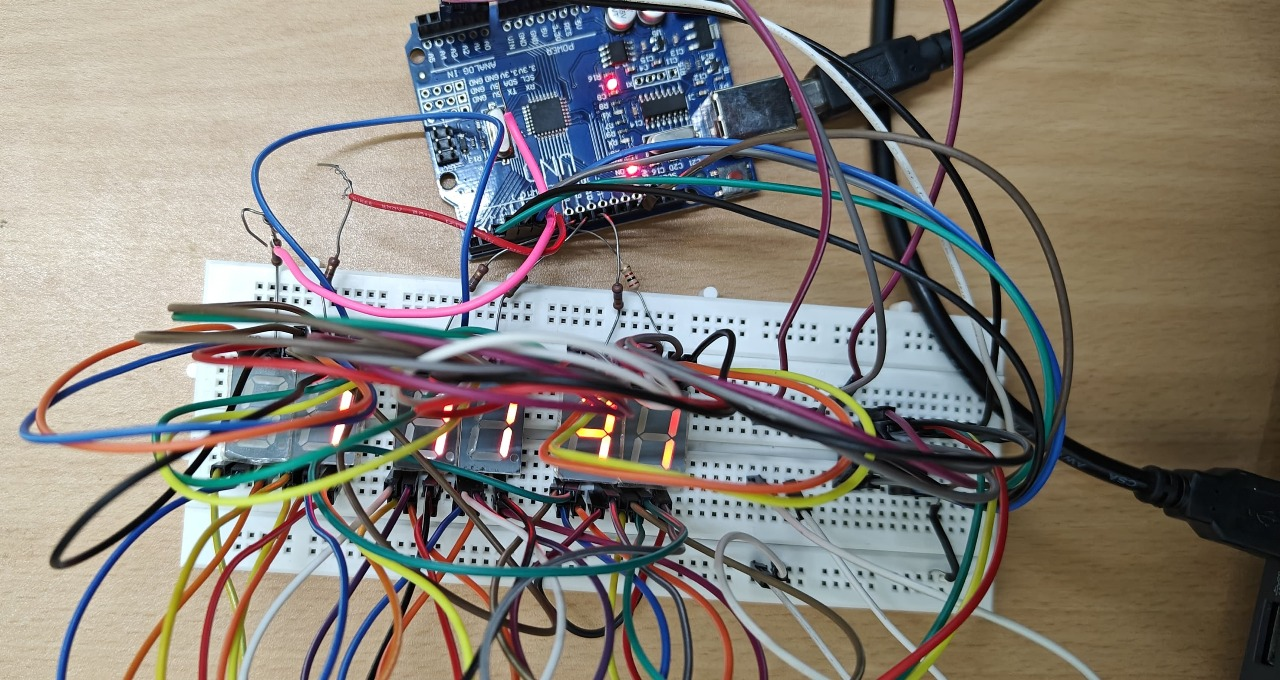
\includegraphics[width=0.8\linewidth]{figure/fig1.png}
    \caption{Circuit Diagram}
    \label{fig:circuit}
\end{figure}


\subsection{7447 IC to 7-Segment Displays}
\begin{itemize}
    \item Connect the output pins (a, b, c, d, e, f, g) of the 7447 IC to the corresponding segments of the 7-segment display.
    \item Use current-limiting resistors $200\ohm$ between the 7447 outputs and the 7-segment display segments.
    \item Connect the common cathode (or anode) of the 7-segment display to GND (or VCC) depending on the type of display.
\end{itemize}
\begin{figure}[H]
    \centering
    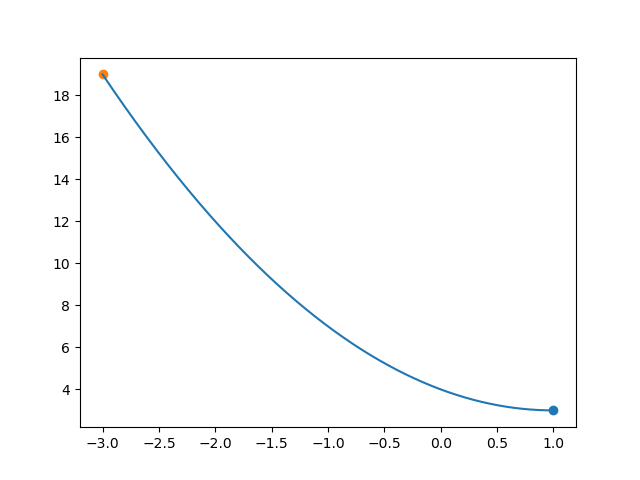
\includegraphics[width=0.8\linewidth]{figure/fig2.png}
    \caption{Circuit Diagram}
    \label{fig:circuit}
\end{figure}


\subsection{Multiplexing}
\begin{itemize}
    \item Use six 7-segment displays for hours, minutes, and seconds.
    \item Use additional 7447 ICs for each digit (total of six 7447 ICs).
    \item Connect the BCD outputs of the Arduino to each 7447 IC in parallel, but use separate Arduino pins to control which digit is active at a time (multiplexing).
    \item Use Arduino digital pins (e.g., D6, D7, D8, D9, D10, D11) to control the common cathode (or anode) of each 7-segment display.
\end{itemize}

\section{Experimental Procedure}
\begin{enumerate}
    \item \textbf{Circuit Connections}:
        \begin{itemize}
            \item Connect the Arduino to the 7447 IC and 7-segment displays as described in the circuit design.
           \item Ensure proper current-limiting resistors are used for the 7-segment displays.
        \end{itemize}
    \item \textbf{Arduino Code}:
        \begin{itemize}
            \item Write and upload the provided Arduino code to implement the digital clock.
        \end{itemize}
    \item \textbf{Testing}:
        \begin{itemize}
            \item Power on the circuit and verify that the displays show the initial time (12:00:00).
            \item Observe the seconds incrementing every second.
            \item Check that the minutes and hours increment correctly.
        \end{itemize}
    \item \textbf{Optional Enhancements}:
        \begin{itemize}
            \item Add push buttons to manually set the hours, minutes, and seconds.
            \item Add an AM/PM indicator for a 12-hour format.
        \end{itemize}
\end{enumerate}
\begin{table}[htbp]
    \centering
    \renewcommand{\arraystretch}{1.2} % Increase row height for better readability
    \caption{Arduino to 7-Segment Display Connections}
    \label{tab:connections}
    \begin{tabular}{cc}
        \toprule
        \textbf{Arduino Pin} & \textbf{7-Segment Display Pin} \\
        \midrule
        2  & a  \\
        3  & b  \\
        4  & c  \\
        5  & d  \\
        6  & e  \\
        7  & f  \\
        8  & g  \\
        \midrule
        9  & COM (1st Display)  \\
        10 & COM (2nd Display)  \\
        11 & COM (3rd Display)  \\
        12 & COM (4th Display)  \\
        A0 & COM (5th Display)  \\
        A1 & COM (6th Display)  \\
        \bottomrule
    \end{tabular}
\end{table}

\section{Arduino Code}
Below is the Arduino code used to implement the digital clock:

\begin{lstlisting}[caption=Arduino Code for Digital Clock]
#include <stdint.h>
#include <stdbool.h>
#include <avr/io.h>       // For AVR microcontrollers
#include <util/delay.h>   // For delay functions

// Define BCD output pins
#define BCD_A 2
#define BCD_B 3
#define BCD_C 4
#define BCD_D 5

// Define digit control pins
const uint8_t digitPins[6] = {6, 7, 8, 9, 10, 11};

// Variables to store time
uint8_t hours = 12;
uint8_t minutes = 0;
uint8_t seconds = 0;

// Function to set a specific pin HIGH or LOW
void setPin(uint8_t pin, bool state) {
    if (state) {
        PORTB |= (1 << pin);  // Set pin HIGH
    } else {
        PORTB &= ~(1 << pin); // Set pin LOW
    }
}

// Function to display a digit on the 7-segment display
void displayDigit(uint8_t digit, uint8_t value) {
    // Set the BCD output based on the value
    setPin(BCD_A, value & 0x01);
    setPin(BCD_B, (value >> 1) & 0x01);
    setPin(BCD_C, (value >> 2) & 0x01);
    setPin(BCD_D, (value >> 3) & 0x01);

    // Turn on the corresponding digit
    setPin(digitPins[digit], true);
    _delay_ms(5); // Display for a short time
    setPin(digitPins[digit], false); // Turn off the digit
}

// Function to update the time
void updateTime() {
    seconds++;
    if (seconds >= 60) {
        seconds = 0;
        minutes++;
        if (minutes >= 60) {
            minutes = 0;
            hours++;
            if (hours >= 24) {
                hours = 0;
            }
        }
    }
}

int main(void) {
    // Set BCD pins as output
    DDRB |= (1 << BCD_A) | (1 << BCD_B) | (1 << BCD_C) | (1 << BCD_D);

    // Set digit control pins as output
    for (uint8_t i = 0; i < 6; i++) {
        DDRB |= (1 << digitPins[i]);
        setPin(digitPins[i], false); // Turn off all digits initially
    }

    // Main loop
    while (1) {
        // Update time every second
        static uint32_t lastTime = 0;
        uint32_t currentTime = millis(); // Implement millis() for your platform
        if (currentTime - lastTime >= 1000) {
            lastTime = currentTime;
            updateTime();
        }

        // Display hours, minutes, and seconds
        displayDigit(0, hours / 10);    // Tens place of hours
        displayDigit(1, hours % 10);    // Units place of hours
        displayDigit(2, minutes / 10);  // Tens place of minutes
        displayDigit(3, minutes % 10);  // Units place of minutes
        displayDigit(4, seconds / 10);  // Tens place of seconds
        displayDigit(5, seconds % 10);  // Units place of seconds
    }

    return 0;
}
\end{lstlisting}

\section{Observations and Results}
\begin{itemize}
    \item The Arduino generated the correct BCD output for each digit.
    \item The 7447 IC successfully decoded the BCD signals and drove the 7-segment displays.
    \item The digital clock displayed the time accurately in the HH:MM:SS format.
    \item Multiplexing ensured that all digits were displayed clearly without flickering.
\end{itemize}

\section{Conclusion}
The digital clock was successfully implemented using an Arduino and the 7447 BCD to 7-segment decoder/driver IC. The circuit accurately displayed time in the HH:MM:SS format. Future enhancements could include adding an AM/PM indicator, alarm functionality, and manual time-setting buttons.

\end{document} 
